\documentclass[conference]{IEEEtran}

\ifCLASSINFOpdf
  \usepackage[pdftex]{graphicx}
\else
  \usepackage[dvips]{graphicx}
\fi
\usepackage{amsmath}
\usepackage{amssymb}
\usepackage{balance}
\usepackage[usenames,dvipsnames,svgnames,table]{xcolor}
\usepackage{algpseudocode}
% \usepackage{minipages}

\newcommand{\compactimg}{\vspace{-10pt}}
\newcommand{\tableref}[1]{Table~\ref{tab:#1}}
\newcommand{\figref}[1]{Figure~\ref{fig:#1}}
\newcommand{\secref}[1]{Section~\ref{sec:#1}}
\newcommand{\algoref}[1]{Algorithm~\ref{algo:#1}}

\hyphenation{}

\begin{document}

\title{Demo Abstract: The OpenChirp Low-Power Wide-Area Network and Ecosystem}
\author{
	\IEEEauthorblockN{Adwait Dongare, Anh Luong, Artur Balanuta, Craig Hesling, Khushboo Bhatia, Anthony Rowe}
	\IEEEauthorblockA{
		Electrical and Computer Engineering Department\\
		Carnegie Mellon University, Pittsburgh PA\\
	}
}

% conference papers do not typically use \thanks and this command
% is locked out in conference mode. If really needed, such as for
% the acknowledgment of grants, issue a \IEEEoverridecommandlockouts
% after \documentclass

% for over three affiliations, or if they all won't fit within the width
% of the page, use this alternative format:
% 
%\author{\IEEEauthorblockN{Michael Shell\IEEEauthorrefmark{1},
%Homer Simpson\IEEEauthorrefmark{2},
%James Kirk\IEEEauthorrefmark{3}, 
%Montgomery Scott\IEEEauthorrefmark{3} and
%Eldon Tyrell\IEEEauthorrefmark{4}}
%\IEEEauthorblockA{\IEEEauthorrefmark{1}School of Electrical and Computer Engineering\\
%Georgia Institute of Technology,
%Atlanta, Georgia 30332--0250\\ Email: see http://www.michaelshell.org/contact.html}
%\IEEEauthorblockA{\IEEEauthorrefmark{2}Twentieth Century Fox, Springfield, USA\\
%Email: homer@thesimpsons.com}
%\IEEEauthorblockA{\IEEEauthorrefmark{3}Starfleet Academy, San Francisco, California 96678-2391\\
%Telephone: (800) 555--1212, Fax: (888) 555--1212}
%\IEEEauthorblockA{\IEEEauthorrefmark{4}Tyrell Inc., 123 Replicant Street, Los Angeles, California 90210--4321}}




% use for special paper notices
%\IEEEspecialpapernotice{(Invited Paper)}




% make the title area
\maketitle

\begin{abstract}

In this demonstartion, we first present OpenChirp, an open-source Low-Power Wide
Area Networking (LPWAN) infrastructure.
We also present LPRAN, a low-cost high-performance software-defined radio
platform.


In this demonstration we present Pulsar, a speed-of-light propagation-aware
time synchronization platform. Pulsar uses ultra-wideband (UWB) radios for
time transfer with each node backed by a chip scale atomic clock (CSAC) that
in combination are able to provide accuracy on the order of 10's of
nanoseconds for indoor applications. The demonstration will show two Pulsar
boards generating a tightly synchronized PPS output that is able to adjust for
the distance between the nodes. Even without communication, the devices
maintain synchronization over multiple seconds due to a stable CSAC clocking
the system.
\end{abstract}

\IEEEpeerreviewmaketitle



% \section{Introduction}
% \label{sec:intro}




\section{System Description}
\label{sec:system}

{\color{red} The first few sections would be the equivalent of the intro.}

Low Power Wide Area Networks (LP-WANs) are increasingly seen as an attractive
communication platform for city-scale Internet-of-Things (IoT) deployments.
They offer the ability to wirelessly connect energy-constrained devices to
gateways over distances of many kilometers. LP-WANs also have power and cost
advantages over alternatives like cellular networks, particularly in
deploy-once, low-maintenance and low throughput sensing applications.

What are we selling?

% the goal of this demo abstract/demo is
% 1. introduce researchers to OC
%       functional city scale data collection framework
%           data scientists ready
%           city scale system integrator
%       LoRa-ready
%           gateways, sensor nodes (cots and custom/lorabug)
%       open source software -> working on the packaging
% 2. channel sniffing w/ LPRAN

Completely open, easy to deploy LPWAN infrastructure

It's here now and how you can you use it.

% OC is for everyone
% 1. scaling -> large scale (city scale)
% 2. open source, security and user friendly
%    bring your own gateway
%    bring your own DB
%    comm technology agnostics
% 3. listening to more than just communcations (LPRAN)
% 4. we deployed across a university campus

Smart home devices are ubiquitous in today's home. However, current indoor
communication technologies while great indoor, has limited ranges and power
hungry.

\begin{figure}[!htb]
    \centering
    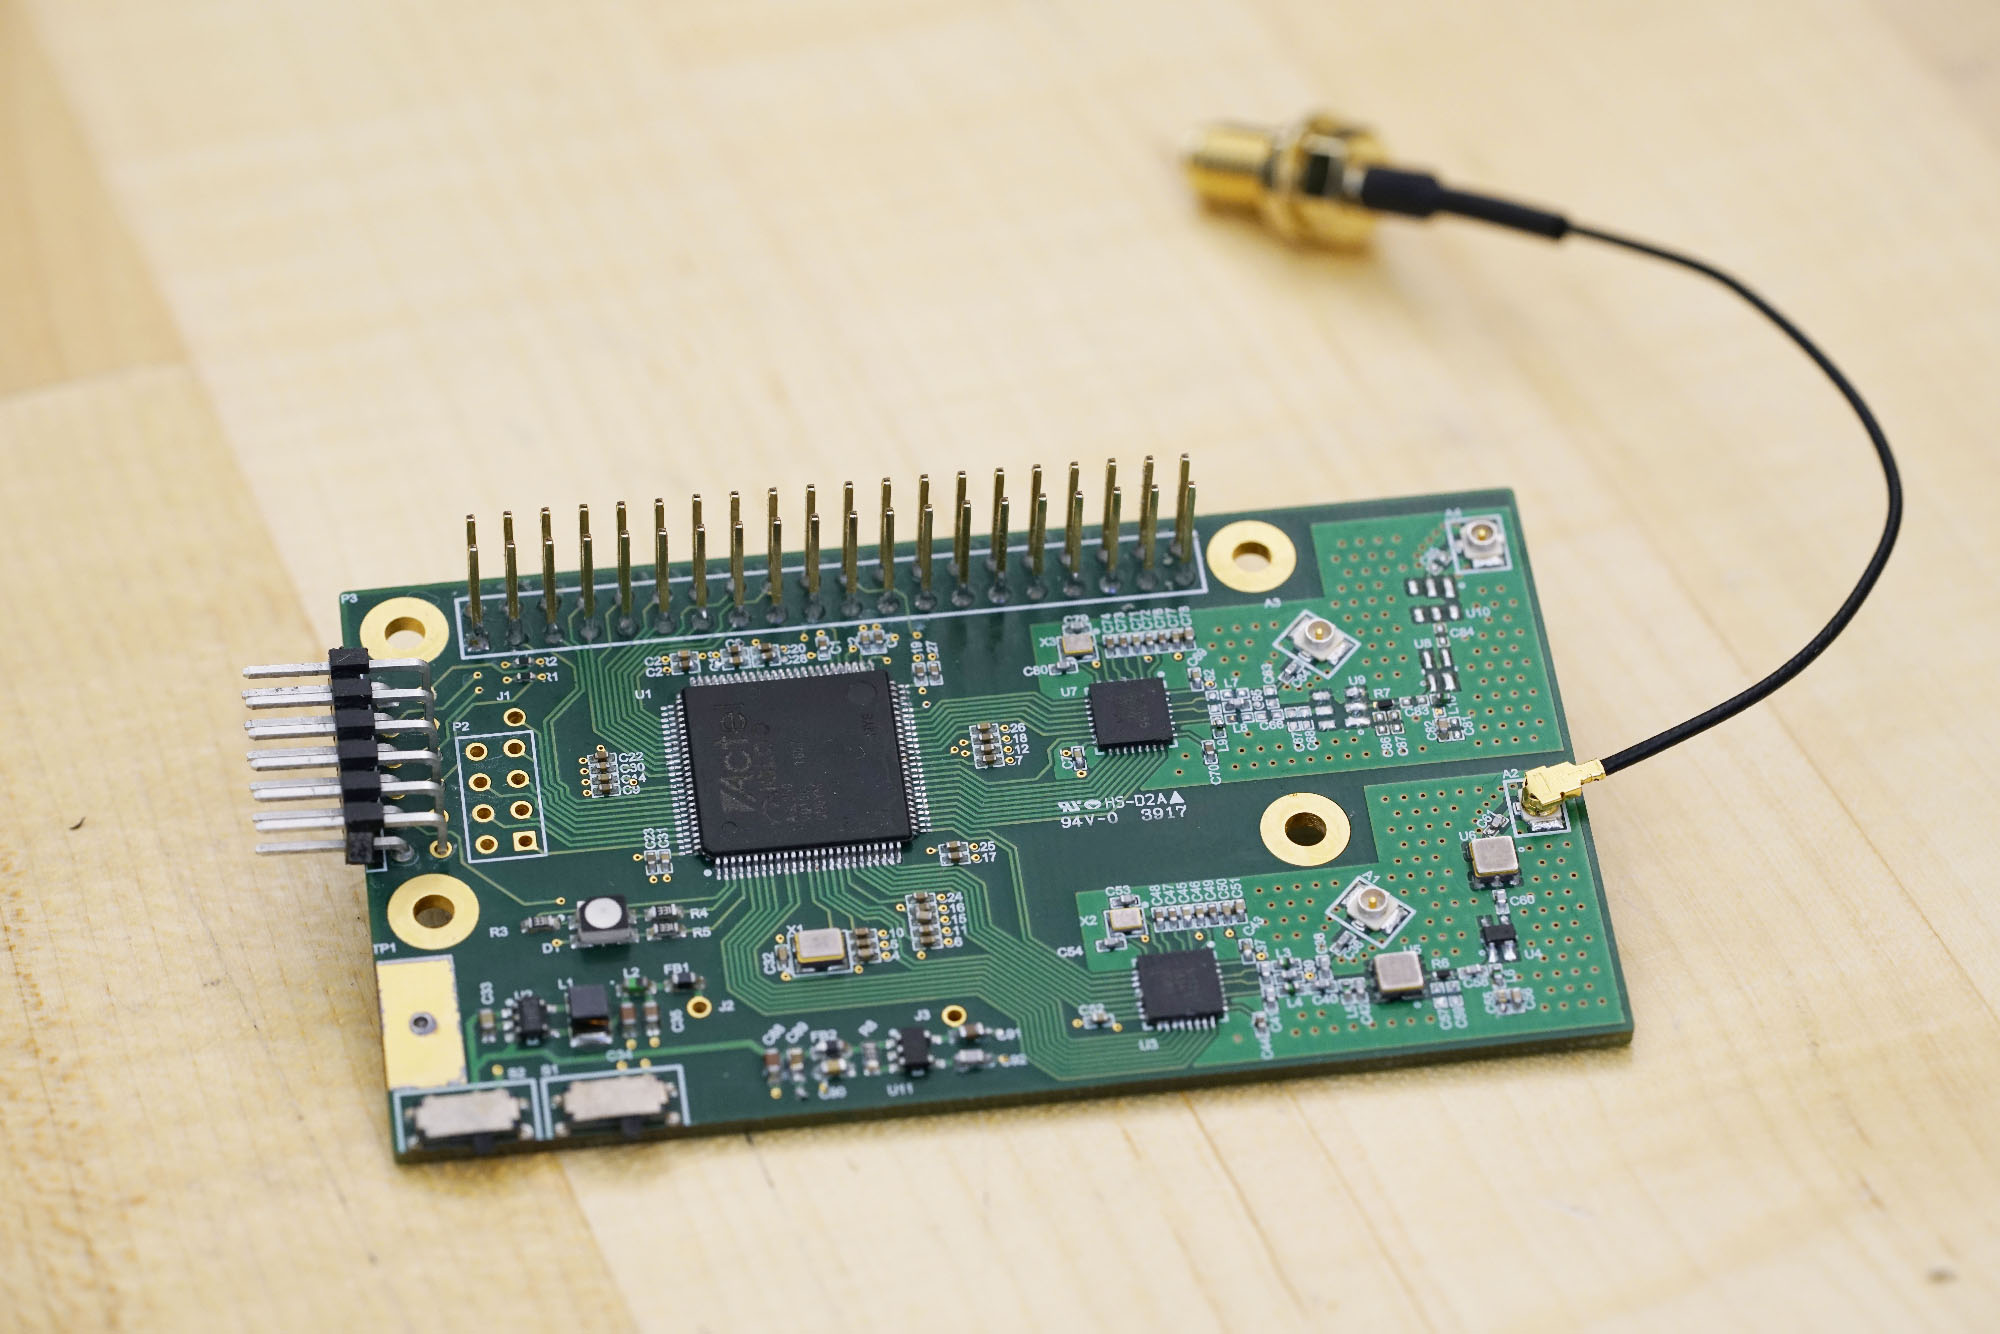
\includegraphics[width=0.5\linewidth]{figures/gw-anon-sm}
    \\
    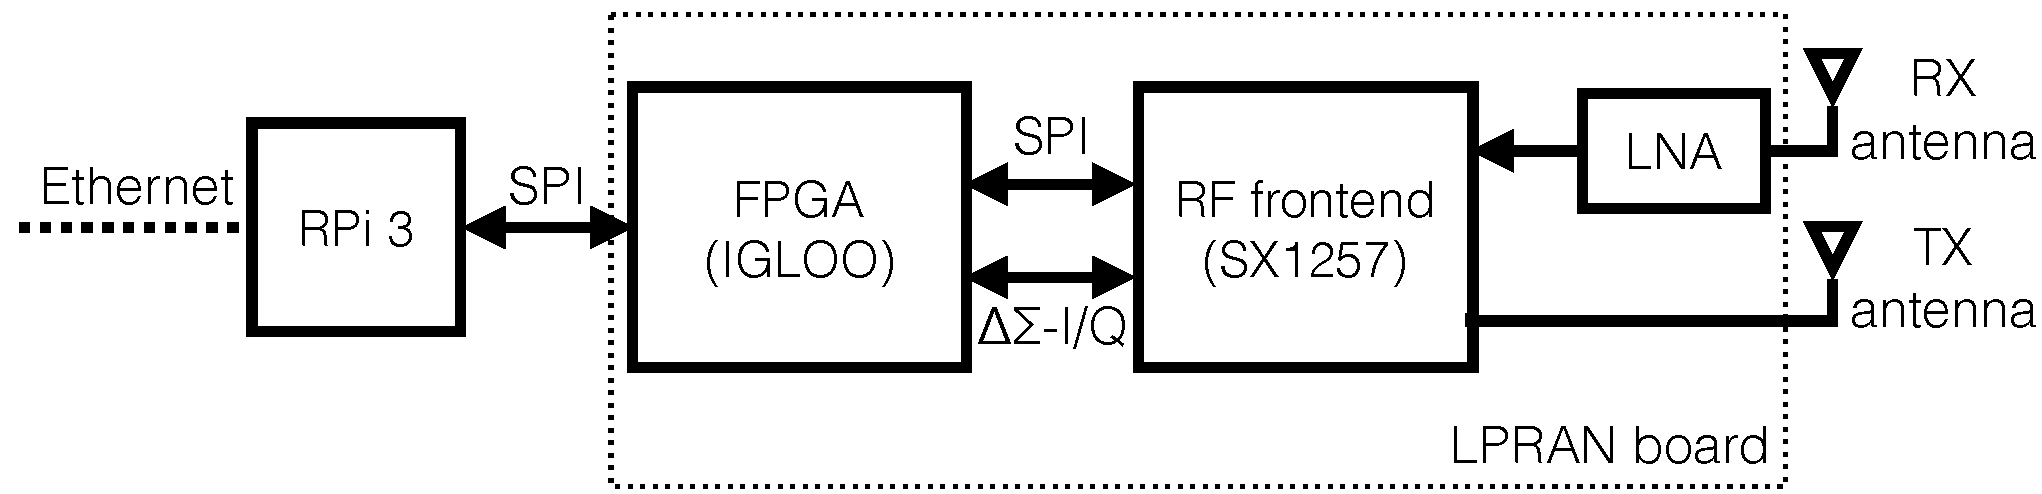
\includegraphics[width=0.8\linewidth]{figures/lpran-block_cropped}
    \caption{{\color{red} Add caption}}
    \label{fig:lpran-photo}
\end{figure}

\begin{figure}[!htb]
    \centering
    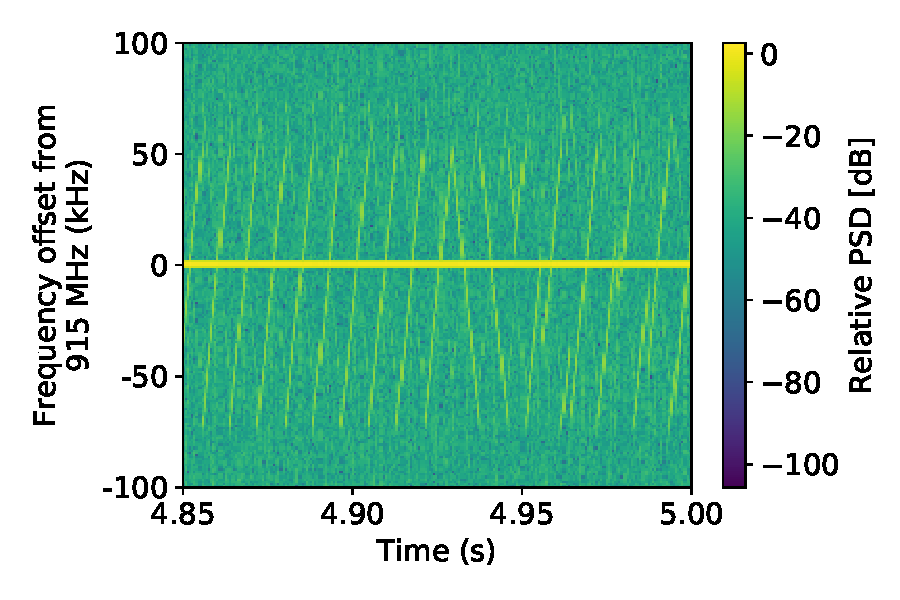
\includegraphics[width=0.8\linewidth]{figures/LPRAN_spectrogram}
    \caption{{\color{red} Add caption}}
    \label{fig:lpran-spectrogram}
\end{figure}

\subsection{OpenChirp Architecture}
\label{sec:oc-arch}

\begin{figure*}[!htb]
    \centering
    \begin{minipage}[b]{.6\textwidth}
        \centering
        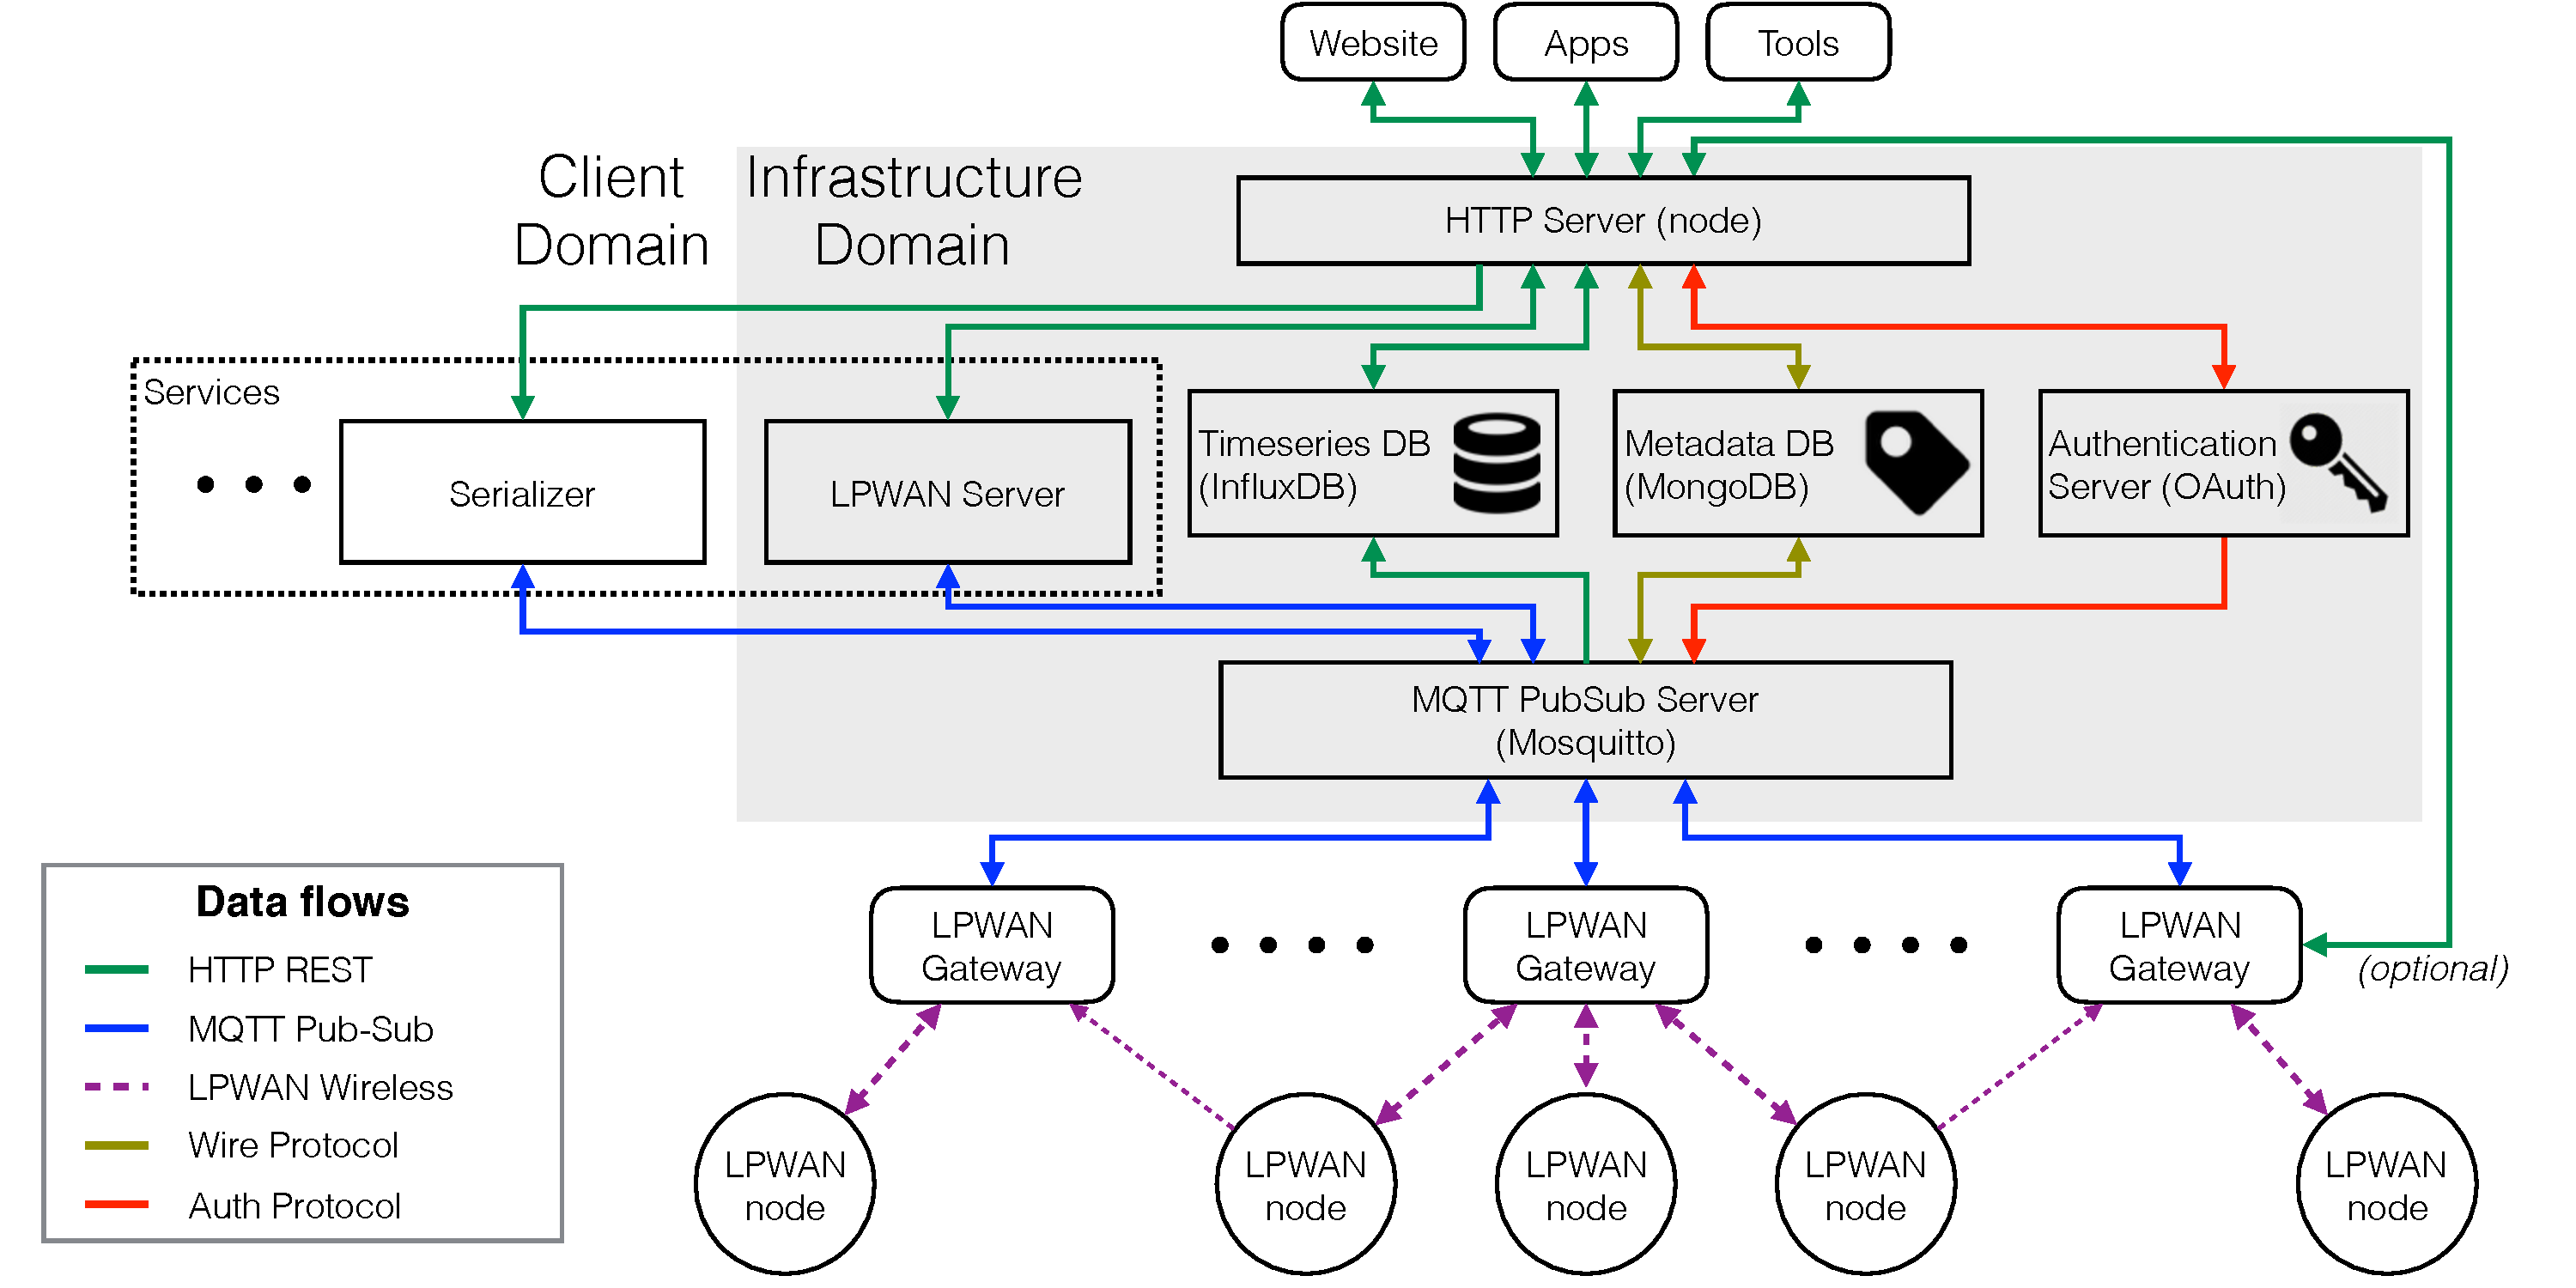
\includegraphics[width=\linewidth]{figures/openChirp_architecture}
        \caption{OpenChirp Architecture}
        \label{fig:oc-arch}
    \end{minipage}%
    \begin{minipage}[b]{.4\textwidth}
        \centering
        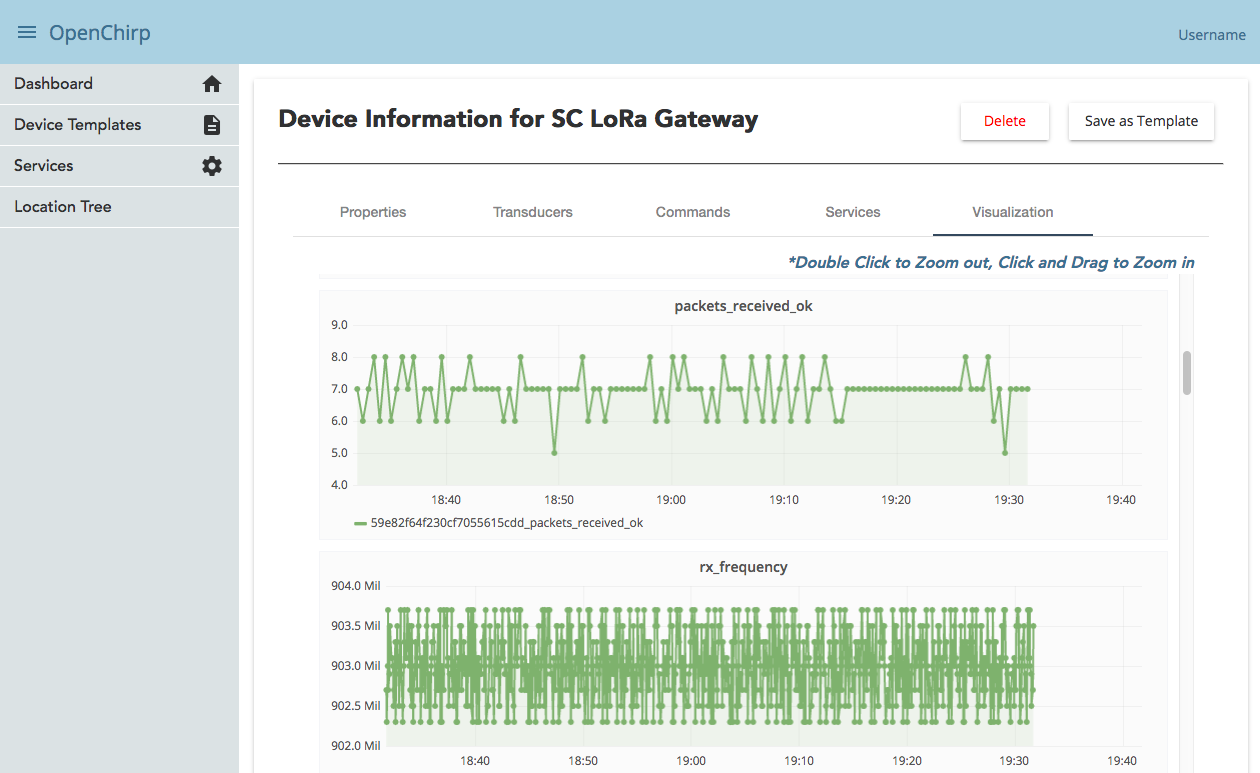
\includegraphics[width=\linewidth]{figures/OC_screenshot}
        \caption{Screenshot of OpenChirp's web interface}
        \label{fig:oc-screenshot}
    \end{minipage}
\end{figure*}

\subsection{LPRAN Architecture}
\label{sec:lpran-arch}



{\color{red} Add system diagram and photo}

\section{Demonstration}
\label{sec:demo}

We demonstrate various software and hardware components to aid the rapid
deployment and management of a LoRa LPWA research network.

\subsection{OpenChirp Interface}
\label{sec:oc-interface-demo}

We will demonstrate the ease and simplicity of adding and managing LoRaWAN
devices as well as gateways using the OpenChirp network interface. We plan to
deploy multiple wireless LoRa devices across the demo area and be able to log
and visualize data using the OpenChirp interface. We use a combination of
commercial off-the-shelf devices (e.g. PyCom LoPy) as well as some custom
LoRaBug devices~\cite{dongare2017openchirp}, that can log sensor values and
perform simple actuations.

An illustration of this setup is shown in {\color{red} CREATE FIGURE FOR THIS
SETUP}.

\subsection{LPRAN Micro-SDR Platform}
\label{sec:lpran-demo}

What do we say here?

We will demonstrate


\section*{Acknowledgment}


The authors would like to thank...


\balance
\bibliographystyle{unsrt}
\bibliography{references} % references.bib is the name of the Bibliography in this case

\section{Demo Requirements}
\label{sec:requirements}

The demonstration requires a power connection (with multiple plugs), a screen,
keyboard and mouse. A stable internet connection would be preferable, but not
essential. This demonstartion will use multiple battery-powered wireless
transmitters in the 868 MHz ISM spectrum.

\end{document}


